\subsection{Experimental Setup}

The experiments are organized around four questions: how much better is KCH-MedRank than strong baselines including a biomedical cross-encoder, does hypergraph structure help or does raw topology introduce noise, do the gains generalize beyond BioASQ, and where does the reranker succeed and fail. The corresponding sections are the main results (Section~\ref{sec:main-results}), structural ablation (Section~\ref{sec:ablation}), robustness diagnostics on PubMedQA and BEIR NFCorpus within this section, and interpretability and error analysis (Section~\ref{sec:interpretability}).

\subsubsection{Dataset and Split}

The primary dataset is \texttt{rag-datasets/rag-mini-bioasq}, containing 4,719 BioASQ-style questions with gold passage-level annotations. We split deterministically by question identifier modulo-5 bucketing: training covers buckets 0--2 (2,832 questions), validation uses bucket 3 (944 questions), and test uses bucket 4 (943 questions). The split is fixed before any model selection. Each question carries multiple gold evidence passages, so Recall@$k$ (macro evidence coverage) is the primary metric.

PubMedQA~\citep{jin2019pubmedqa} provides a secondary diagnostic in the yes/no/maybe QA format with strong first-hit retrieval. BEIR NFCorpus~\citep{thakur2021beir} is an external retrieval-only robustness test. MeSH, entity, and hypergraph features are not built for NFCorpus, so only retrieval-feature LambdaMART is compared there.

\subsubsection{Baselines}

First-stage retrievers include BM25, dense biomedical retrieval, original Hybrid RRF (BM25 and dense with equal weights), fielded BM25 with MeSH expansion, MedCPT dual-encoder retrieval, and enhanced Hybrid RRF in the w122 configuration selected on validation Recall@100.

Reranking baselines span the strongest available semantic model down to the simplest retrieval-only ranker: MedCPT Cross-Encoder~\citep{jin2023medcpt} on the same enhanced candidate pool, retrieval-feature-only LambdaMART with no biomedical knowledge, flat biomedical knowledge LambdaMART with all knowledge features but no graph structure, pairwise graph LTR, hypergraph LTR without medical knowledge, and full KCH-MedRank.

\subsubsection{Evaluation Protocol}

Metrics are Recall@$k$, Hit@$k$, MRR@$k$, and nDCG@$k$ for $k \in \{1,3,5,10,20,50,100\}$. Recall@$k$ is macro evidence coverage: per question, the fraction of its gold passages in the top $k$, averaged across questions. Statistical significance comes from paired bootstrap with 10,000 resamples and a fixed random seed. All model selection uses validation metrics only; the test split is evaluated exactly once.

A hard reranking subset isolates 65 test questions where the enhanced Hybrid RRF candidate pool contains gold evidence in the top 100 but misses every gold passage in the top 10. On this subset the baseline has Recall@10 of 0 by construction. Passing it means knowledge features rescued evidence that retrieval signals alone could not.

\paragraph{Concept Normalization Diagnostic.}
To assess the synonym normalization module, we compare three controlled configurations under the same validation-set constraints: (i) the retrieval-feature LTR baseline, (ii) KCH-MedRank with base flat knowledge features (without synonym-aware augmentation), and (iii) KCH-MedRank with full synonym-aware features. The comparison uses the validation split only (bucket 3, 944 questions) to maintain test-set integrity. Additionally, we measure a synonym-coverage metric: among all question--gold-passage pairs in the test set, the fraction for which exact entity matching yields zero overlap while normalized variant matching recovers a non-zero overlap. This metric directly quantifies the gap that the normalization module is designed to bridge.

\begin{table}[t]
\centering
\small
\caption{Validation-selected enhanced candidate generation. Fusion weights are selected only on the validation split.}
\label{tab:enhanced-candidate-selection}
\begin{tabular}{lrrrrrr}
\toprule
Fusion run & BM25 & Dense & Fielded BM25 & MedCPT DE & Val. R@100 & Test R@100 \\
\midrule
Original Hybrid & 1.0 & 1.0 & 0.0 & 0.0 & 0.6325 & 0.6077 \\
w052 & 1.0 & 1.0 & 0.5 & 0.2 & 0.6391 & 0.6163 \\
w084 & 1.0 & 1.0 & 0.8 & 0.4 & 0.7329 & 0.7084 \\
w102 & 1.0 & 1.0 & 1.0 & 0.2 & 0.7529 & 0.7285 \\
w122, selected & 1.0 & 1.0 & 1.2 & 0.2 & 0.7568 & 0.7388 \\
\bottomrule
\end{tabular}
\end{table}


\begin{figure}[htbp]
\centering
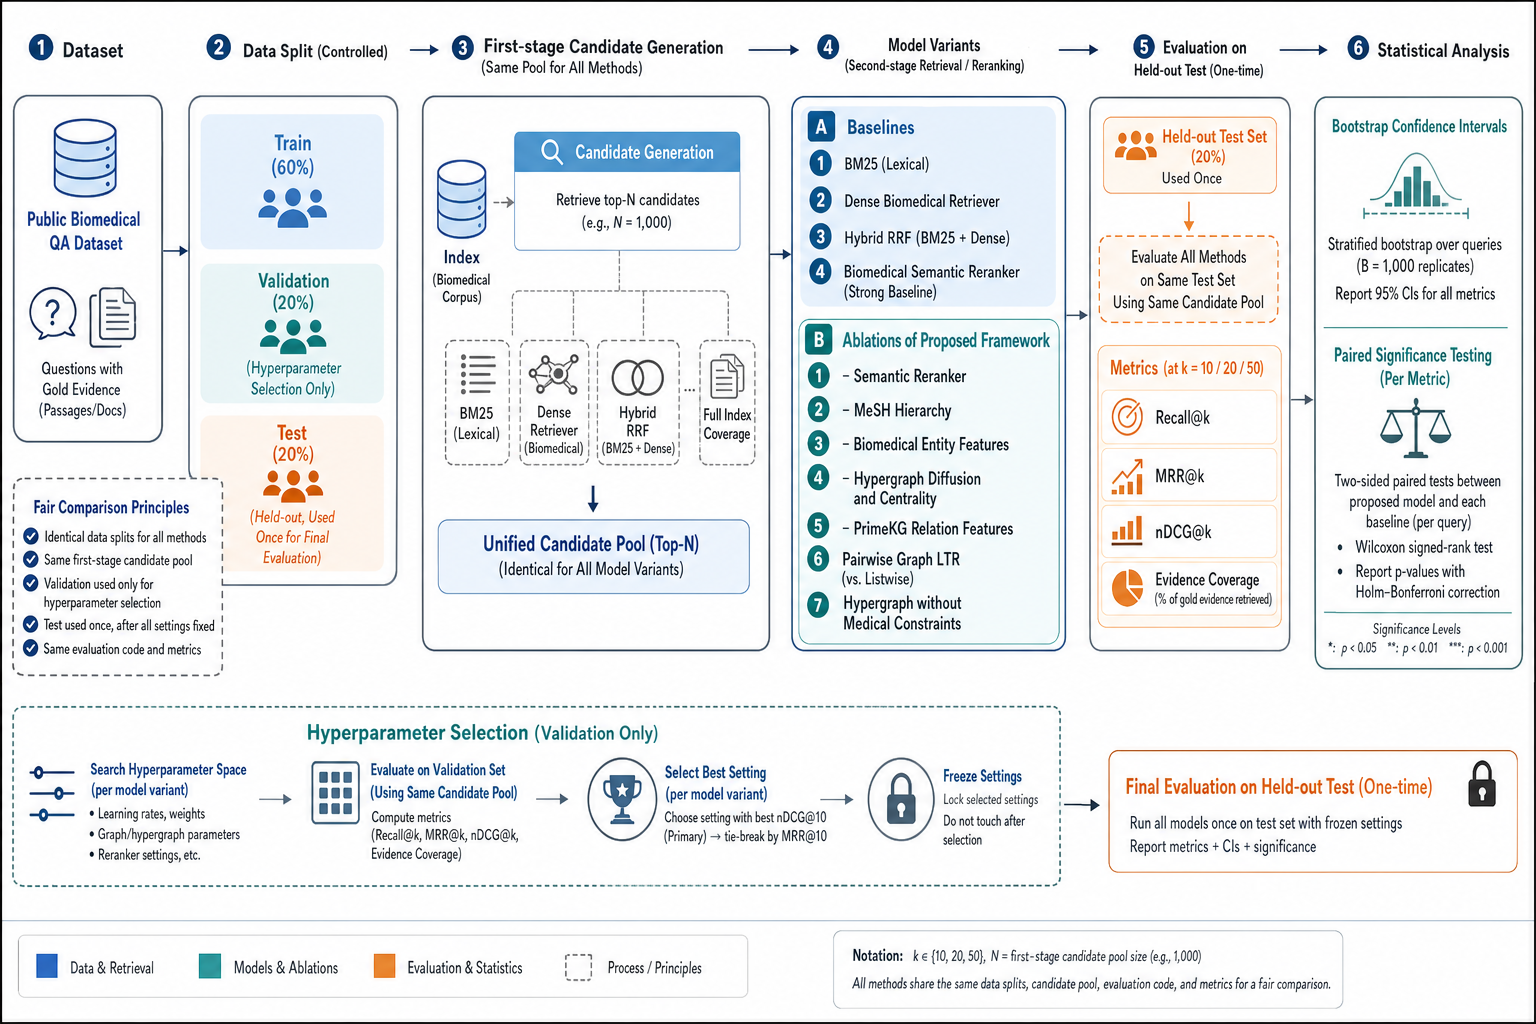
\includegraphics[width=0.98\linewidth]{figures/gpt_image2_figure_04.png}
\caption{Controlled experimental design: candidate generation, reranking baselines, structural ablations, validation-only model selection, and paired statistical testing.}
\label{fig:gpt-experimental-design}
\end{figure}
